\documentclass{article}
\usepackage[utf8]{inputenc}
\usepackage{graphicx}

\title{FPGA Example Design: Xilinx Zynq Board}
\author{JITX Team}
\date{\today}

\begin{document}

\maketitle

\section{Project Goals and Future Prospects}

\subsection{Primary Objectives}
\begin{itemize}
    \item Develop an FPGA design of moderate complexity using JITX, serving as a comprehensive overview of the tool's capabilities.
    \item Utilize this design as a stress test to identify and resolve bugs in the JITX toolchain, while ensuring adequate performance.
    \item Create a compelling marketing asset: A Zynq-based board represents a significant engineering challenge. Successfully implementing this design demonstrates JITX's ability to handle complex projects, appealing to professionals already working with the Zynq platform and those engaged in projects of similar complexity.
\end{itemize}

\subsection{Future Enhancements}
\begin{itemize}
    \item Refactor the codebase to improve reusability and parameterization, with the ultimate goal of integrating it into the JSL library.
    \item Expand the design to interface with a VPX backplane, contingent upon the development of a VPX backplane generator. This addition would transform the project into a highly attractive example for specific industry players, such as Lockheed-Martin.
    \item Potential to evolve into a world-class VPX backplane solution, further enhancing JITX's market position in specialized, high-performance computing applications.
\end{itemize}

\section{Architecture}

Here's the key components of the design:
\begin{enumerate}
    \item Xilinx Zynq SoC
    \item DDR4 memory
    \item Flash memory for bring-up
    \item ADC input to the FPGA, fed from a Coax connector
    \item HDMI output
    \item USB 2.0 and JTAG interface for bring-up and debugging
\end{enumerate}

\begin{figure}
    \centering
    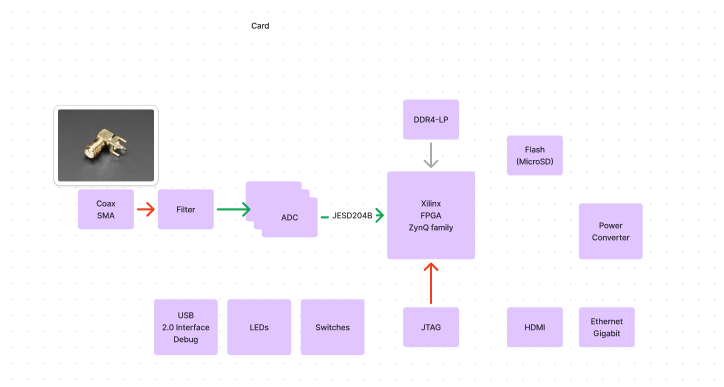
\includegraphics[width=0.8\textwidth]{../pics/block-diagram.png}
    \caption{Block diagram of the Zynq FPGA-based Design}
    \label{fig:fpga-block-diagram}
\end{figure}

\section{Part Selection}

\subsection{FPGA device}

Considering {\em XCZU1CG-1UBVA494I}:
\begin{itemize}
    \item Driven by need to support DDR4 memory. Lower-cost Zynq-7000 series only support up to DDR3.
    \item Lowest-cost Zynq Ultrascale+ part in stock on Digikey is XCZU1CG-1UBVA494I: \$292.52
    \item Dual core Arm Cortex-A53 (APU) + Dual core Arm Cortex-R5F (RPU)
    \item 81,900 Logic cells.
    \item 170 PS (Processing System) I/O, supporting 32-bit DDR4 only.
    \item 24 HD (High-Density) I/O. 58 HP (High-Performance) I/O.
\end{itemize}

\subsubsection{Supported DDR4 memory speed}
\begin{itemize}
\item For UBVA494 package
\item For 1-rank components: Min 1000 Mb/s. Max 1866 Mb/s
\item For 2-rank components w/ dual-rank package: Min 1000 Mb/s. Max 1600 Mb/s.
\item For 2-rank components w/ single-rank package: Min 1000 Mb/s. Max 1333 Mb/s.
\end{itemize}
See Table 30 in {\em ds925-zynq-ultrascale-dc-ac-switching-characteristics.pdf}. 


\subsubsection{Selecting a memory configuration}
\begin{enumerate}
\item Memory Type: DDR4
\item Total Capacity: 4 GB (32 Gb)
\item Data Width: 32-bit
\item Component Configuration: 2 x 16Gb DDR4 chips (x16 width each)
\item Single rank
\item No ECC
\end{enumerate}

This configuration uses two 16 Gb (2 GB) DDR4 chips, each with a x16 interface, to create a 32-bit wide data bus with a total capacity of 4 GB. Keep the design simple using a single rank configuration, which also allows utilization of full 1866 Mb/s speed. See Table 17-1 in {\em ug1085-memory-excerpt.pdf}. 

\subsection{Memory ICs}

Based on above requirements Micron {\em MT40A1G16TD-062E AIT:F} seems to work. Currently in-stock at Digikey for \$18.73.

\section{Selecting an ADC}

The ZynQ has MIO (Multiplexed I/O) and EMIO (Extended Multipled I/O) pins, with SPI available on both. 

The datasheet says that SPI performance is better using the MIO pins. (Table 28-2 in technical reference manual). 

The MIO pins can be configured for 1.8V or 3.3V signaling. (Chapter 28 in technical reference manual.)

Consider the Analog Devices {\em AD7091R-8BCPZ-RL7}.

\begin{itemize}
\item 12-bit input
\item 1M samples per second
\item SPI interface.
\item Voltage 2.09V ~ 5.25V
\end{itemize}

In stock for \$9.93 at Digikey.

\end{document}
